\chapter{Planteamiento del Problema}
\section{Descripción de la Realidad Problemática}

La industria global de cuidado de la piel ha experimentado un crecimiento sostenido en los últimos años, como se puede ver en la Figura \ref{1:fig1}. En 2023, se estimó que el mercado mundial generó ingresos de aproximadamente 181.2 mil millones de dólares estadounidenses, con proyecciones que indican un aumento a más de 210 mil millones para 2028 . Este crecimiento refleja una tasa compuesta anual significativa, impulsada por la creciente conciencia sobre la importancia del cuidado de la piel y la demanda de productos innovadores. \parencite{databridge2024}

\begin{figure}[!ht]
	\begin{center}
		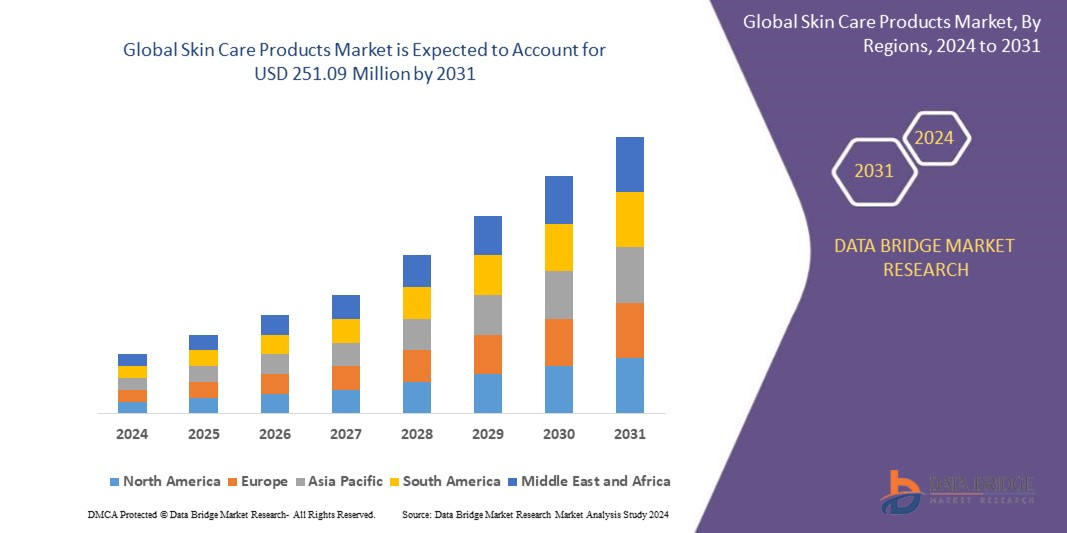
\includegraphics[width=1\textwidth]{1/figures/GlobalSkinCareProductsMarket.jpg}
		\caption[Mercado mundial de productos para el cuidado de la piel: tendencias de la industria y pronóstico hasta 2031]{Mercado mundial de productos para el cuidado de la piel: tendencias de la industria y pronóstico hasta 2031.\\
			Fuente: \cite{databridge2024}. \citetitle{databridge2024}.}
		\label{1:fig1}
	\end{center}
\end{figure}

Dentro de este mercado, el segmento de cuidado facial representa la mayor proporción de ingresos, como se puede ver en la Figura \ref{1:fig2}alcanzando aproximadamente 108.94 mil millones de dólares en 2023 . Este segmento incluye productos como cremas hidratantes, sueros antiarrugas y tratamientos despigmentantes, dirigidos a abordar preocupaciones estéticas como arrugas dilatados y manchas faciales. \parencite{statista2023segment}

\begin{figure}[!ht]
	\begin{center}
		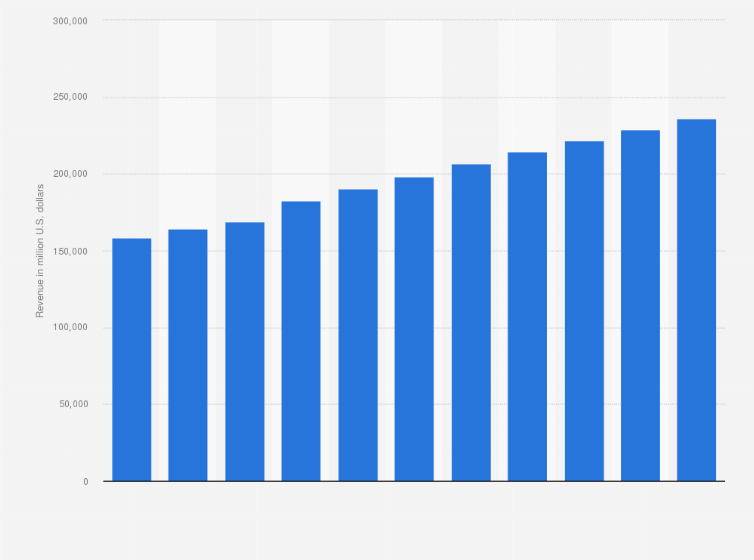
\includegraphics[width=1\textwidth]{1/figures/cap1global.png}
		\caption[Ingresos del mercado mundial del cuidado de la piel de 2020 a 2030 (en millones de dólares estadounidenses)]{Ingresos del mercado mundial del cuidado de la piel de 2020 a 2030 (en millones de dólares estadounidenses).\\
			Fuente: \cite{statista2023global}. \citetitle{statista2023global}.}
		\label{1:fig2}
	\end{center}
\end{figure}

Estados Unidos se posiciona como el mercado más lucrativo en la industria del cuidado de la piel. En 2023, el mercado estadounidense generó ingresos cercanos a 24 mil millones de dólares, superando a otros países como Japón y China . Se proyecta que para 2025, los ingresos alcancen los 26.01 mil millones de dólares, con una tasa de crecimiento anual compuesta del 4.53\% entre 2025 y 2029. \parencite{statista2023us}

El segmento de cuidado facial domina el mercado estadounidense, lo podemos ver en la Figura \ref{1:fig3}, representando la mayor parte de las ventas. En 2023, las ventas de productos para el cuidado de la piel en Estados Unidos superaron los 23.5 mil millones de dólares, con el segmento facial contribuyendo significativamente a esta cifra. \parencite{statista2025usforecast}

\begin{figure}[!ht]
	\begin{center}
		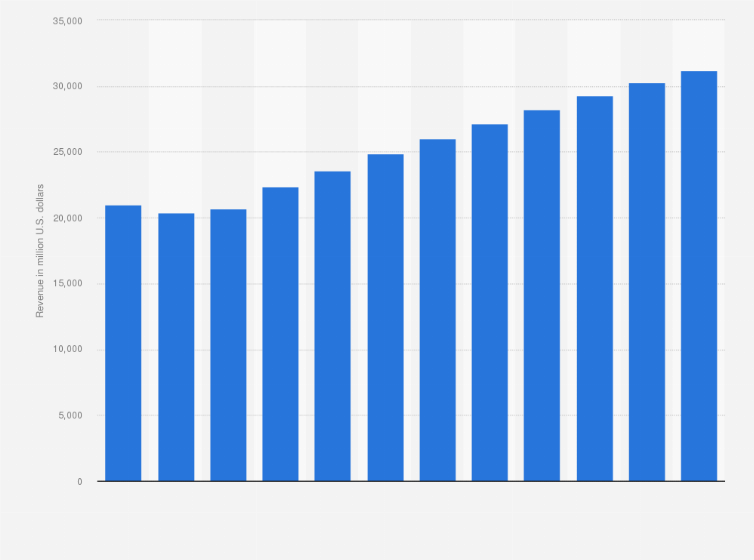
\includegraphics[width=1\textwidth]{1/figures/cap1usa.png}
		\caption[Ingresos del mercado del cuidado de la piel en Estados Unidos de 2019 a 2030 (en millones de dólares estadounidenses)]{Ingresos del mercado del cuidado de la piel en Estados Unidos de 2019 a 2030 (en millones de dólares estadounidenses).\\
			Fuente: \cite{statista2023us}. \citetitle{statista2023us}.}
		\label{1:fig3}
	\end{center}
\end{figure}

El mercado peruano de belleza y cuidado personal también ha mostrado un crecimiento notable. En 2023, se estimó que el mercado generó ingresos de aproximadamente 2.94 mil millones de dólares, con una tasa de crecimiento anual compuesta proyectada del 4.60\% . Dentro de este mercado, el segmento de cuidado personal, que incluye productos para el cuidado de la piel, representa una proporción significativa, con un volumen estimado de 1.72 mil millones de dólares en 2025. \parencite{statista2023peru}

En el Perú, el mercado de belleza y cuidado personal ha mostrado un crecimiento sostenido, como se ve en la Infografía de la Figura \ref{1:fig4}, alcanzando los 2,240 millones de soles en ventas durante 2023, con proyecciones favorables para los próximos años, según datos proporcionados por la Cámara de Comercio de Lima (CCL). Este comportamiento refleja una creciente preocupación de los consumidores por el cuidado estético, especialmente en segmentos como el cuidado facial y productos anti-edad. \parencite{elperuano2025belleza}

\begin{figure}[!ht]
	\begin{center}
		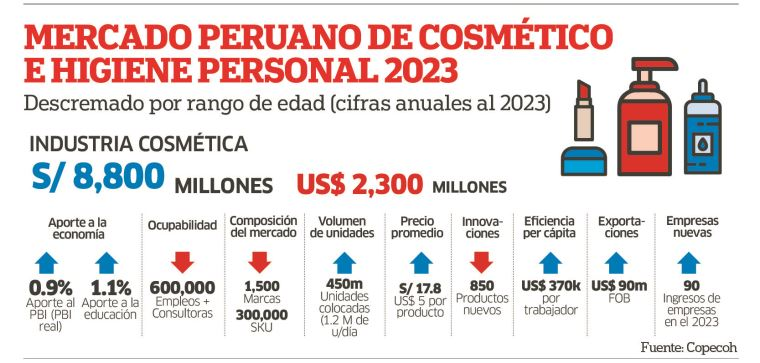
\includegraphics[width=1\textwidth]{1/figures/careperu.jpg}
		\caption[Infografía de la Proyección del Mercado Cosmético e Higiene Personal en Perú]{Infografía de la Proyección del Mercado Cosmético e Higiene Personal en Perú.\\
			Fuente: \cite{elperuano2025belleza}. \citetitle{elperuano2025belleza}.}
		\label{1:fig4}
	\end{center}
\end{figure}

A pesar de la amplia disponibilidad de productos y tratamientos, persisten desafíos en la evaluación precisa y personalizada de problemas cutáneos. La falta de herramientas tecnológicas avanzadas dificulta el análisis cuantitativo de características morfológicas de la piel, como arrugas y manchas. Actualmente, muchos diagnósticos dependen de observaciones manuales, lo que puede llevar a evaluaciones subjetivas y tratamientos menos efectivos. \parencite{esteva2017}

Investigaciones recientes han demostrado el potencial de las redes neuronales convolucionales (CNN) en la clasificación y análisis de imágenes de la piel. Un estudio destacado por Andre Esteva y colaboradores utilizó una base de datos de 129,450 imágenes clínicas para entrenar una CNN capaz de clasificar lesiones cutáneas con una precisión comparable a la de dermatólogos certificados . Este avance sugiere que las CNN pueden ser herramientas valiosas para mejorar la precisión en la evaluación de características cutáneas y el desarrollo de tratamientos personalizados. \parencite{clevelandclinic2023}

El envejecimiento de la piel es una preocupación común entre adultos jóvenes. Según la Clínica Cleveland, las líneas finas pueden comenzar a aparecer después de los 25 años, y las arrugas se vuelven más prominentes entre los 40 y 55 años . Además, un estudio en Corea del Sur encontró que el 33\% de los adultos jóvenes presentaban algún grado de arrugas faciales, porcentaje que aumentaba al 87.8\% en personas de mediana edad y al 100\% en adultos mayores. \parencite{lee2008}

\section{Formulación del Problema}

\subsection{Problema General}
PG: \newcommand{\ProblemaGeneral}{
¿De qué manera pueden las Redes Neuronales Convolucionales segmentar de forma eficiente las características morfológicas faciales?
}
\ProblemaGeneral

\subsection{Problemas Específicos}
\newcommand{\Pbone}{
¿De qué fuentes se obtendrán los datos necesarios para el entrenamiento y la validación del sistema de segmentación?
}
\newcommand{\Pbtwo}{
¿Cuáles serán las etapas y métodos para el desarrollo del sistema de segmentación basado en Redes Neuronales Convolucionales?
}
\newcommand{\Pbthree}{
¿Qué métricas, procedimientos y criterios se emplearán para evaluar la eficiencia y seleccionar el modelo de segmentación más adecuado en la detección de arrugas, manchas y otras características morfológicas faciales?
}
\newcommand{\Pbfour}{
¿Cómo se implementará un sistema de segmentación morfológica facial en tiempo real utilizando redes neuronales convolucionales con mecanismos de atención?
}

\begin{itemize}
	\item PE1: {\Pbone}
	\item PE2: {\Pbtwo}
	\item PE3: {\Pbthree}
	\item PE4: {\Pbfour}
\end{itemize}

\section{Objetivos de la Investigación}
A continuación, se presentan el objetivo general y los objetivos específicos.
\subsection{Objetivo General}
OG: \newcommand{\ObjetivoGeneral}{
Desarrollar un Sistema de Segmentación de Características Morfológicas Faciales, enfocado en la detección de arrugas y manchas, mediante el uso de Redes Neuronales Convolucionales.
}
\ObjetivoGeneral
\subsection{Objetivos Específicos}
\newcommand{\Objone}{
Recopilar y preprocesar un conjunto representativo de imágenes faciales, que incluya diversidad en tipos de piel y afecciones cutáneas, para su utilización en el entrenamiento y validación del sistema de segmentación.
}

\newcommand{\Objtwo}{
Diseñar, desarrollar e implementar un sistema de segmentación basado en Redes Neuronales Convolucionales, orientado a la detección precisa de características morfológicas faciales, específicamente arrugas y manchas.
}

\newcommand{\Objthree}{
Definir e implementar métricas de evaluación cuantitativas para medir la efectividad del sistema de segmentación, y comparar el desempeño de diferentes arquitecturas de Redes Neuronales Convolucionales y técnicas de Aprendizaje Profundo, con el objetivo de seleccionar el modelo que logre el mejor equilibrio entre precisión y eficiencia computacional.
}
\newcommand{\Objfour}{
Implementar un sistema de segmentación morfológica facial en tiempo real utilizando Redes Neuronales Convolucionales con mecanismos de atención, para detectar eficientemente arrugas y manchas.
}
\begin{itemize}
	\item OE1: {\Objone}
	\item OE2: {\Objtwo}
	\item OE3: {\Objthree}
	\item OE4: {\Objfour}
\end{itemize}


\section{Justificación de la Investigación}

\subsection{Teórica}

Este estudio plantea el diseño y desarrollo de un modelo basado en redes neuronales convolucionales (CNN), las cuales han demostrado un rendimiento sobresaliente en tareas de clasificación, detección y segmentación de imágenes, especialmente en contextos médicos y biomédicos \parencite{esteva2017}. Las CNN son particularmente eficaces al capturar patrones espaciales jerárquicos dentro de imágenes, lo que las convierte en herramientas idóneas para analizar características morfológicas complejas como arrugas, poros dilatados y manchas cutáneas.

La aplicación de estas arquitecturas de aprendizaje profundo al campo de la dermatología computacional responde a una creciente necesidad de automatización y precisión diagnóstica en el análisis de imágenes de piel, tanto en contextos clínicos como cosméticos. En la actualidad, gran parte del diagnóstico dermatológico depende de la experiencia visual subjetiva de los profesionales de la salud o de tecnologías que no permiten una segmentación detallada de las estructuras faciales. Esta falta de precisión dificulta el monitoreo objetivo de tratamientos dermatológicos o estéticos y limita la personalización de los mismos \parencite{lee2020}.

Mediante la incorporación de técnicas de deep learning en el procesamiento de imágenes faciales, este estudio busca contribuir no solo al perfeccionamiento de herramientas tecnológicas aplicadas al cuidado personal, sino también al cuerpo de conocimiento que existe en la intersección entre inteligencia artificial y ciencias de la salud. El uso de CNN permite abordar tareas de segmentación con una granularidad que supera los métodos tradicionales, facilitando la detección temprana de signos de envejecimiento, hiperpigmentaciones o alteraciones cutáneas superficiales que podrían ser indicativas de patologías subyacentes o simplemente influir en la percepción estética del rostro \parencite{phillips2020, gao2018}.

Además, este tipo de investigación fortalece el desarrollo de sistemas inteligentes con capacidad de autoaprendizaje, lo cual tiene implicancias directas en la industria cosmética, ya que permitiría la creación de aplicaciones móviles o plataformas web capaces de ofrecer diagnósticos preliminares, seguimiento de tratamientos, o recomendaciones personalizadas basadas en el análisis visual de la piel del usuario. Así, el presente estudio no solo aporta al desarrollo académico en el ámbito de la inteligencia artificial aplicada, sino también al diseño de soluciones tecnológicas que puedan ser integradas en productos de uso cotidiano.

\subsection{Práctica}
Desde un enfoque aplicado, el sistema de segmentación morfológica propuesto presenta un alto potencial de impacto en diversos sectores, particularmente en la industria cosmética, dermatológica y médica. En el ámbito cosmético, esta herramienta puede emplearse para ofrecer evaluaciones automáticas de la piel que guíen la selección de productos según las condiciones faciales específicas del usuario, como arrugas finas, hiperpigmentaciones o poros dilatados. Esto representa una oportunidad significativa para la personalización masiva de productos, mejorando la experiencia del consumidor y fortaleciendo la fidelidad hacia las marcas que integren inteligencia artificial en sus soluciones.

En dermatología, el sistema puede complementar la labor médica mediante la detección temprana y precisa de imperfecciones cutáneas, contribuyendo al diagnóstico preventivo de condiciones dérmicas y al monitoreo del progreso de tratamientos tópicos o procedimientos estéticos no invasivos. Esta automatización reduce la carga de trabajo en clínicas y consultorios, optimiza los tiempos de atención, y proporciona una evaluación objetiva, reproducible y cuantificable del estado de la piel, mitigando la variabilidad que suele existir entre profesionales humanos \parencite{huang2020}.

Adicionalmente, en el sector médico y tecnológico, esta herramienta puede integrarse en aplicaciones móviles, cabinas inteligentes o espejos digitales, abriendo nuevas posibilidades para el desarrollo de interfaces humano-máquina que permitan realizar escaneos faciales sin contacto y de manera remota. Este enfoque puede ser especialmente valioso en contextos rurales o con acceso limitado a dermatólogos especializados.

En suma, el sistema no solo aporta valor tecnológico al automatizar una tarea compleja como la segmentación de estructuras faciales, sino que también genera ventajas competitivas en la industria de la belleza y la salud, al permitir ofrecer servicios personalizados, más eficientes y de mayor calidad.

\subsection{Metodológica}

Desde el punto de vista metodológico, este proyecto se sustenta en la utilización de redes neuronales convolucionales (CNN), una arquitectura de deep learning ampliamente validada en tareas de segmentación y clasificación de imágenes biomédicas \parencite{ronneberger2015}. Su capacidad para identificar patrones espaciales jerárquicos y aprender representaciones discriminativas las convierte en herramientas particularmente efectivas para el análisis morfológico de imágenes faciales.

La metodología propuesta se apoya en la selección de arquitecturas CNN previamente documentadas, como U-Net, ResNet o EfficientNet, que ofrecen robustez y flexibilidad para abordar problemas de segmentación pixel a pixel. Este enfoque no solo mejora la precisión y reproducibilidad de los resultados, sino que también permite comparar el rendimiento entre distintas configuraciones, hiperparámetros y funciones de pérdida, facilitando así una exploración científica profunda sobre cuál es el modelo más eficiente para detectar y segmentar características específicas como arrugas, manchas y poros.

El uso de datasets etiquetados y técnicas de data augmentation permitirá entrenar modelos capaces de generalizar a diferentes condiciones de iluminación, tonalidades de piel y tipos de imperfecciones. Asimismo, el análisis de métricas cuantitativas como IoU (Intersection over Union), Dice Coefficient, precisión y recall, aportará un marco sistemático para validar y comparar las aproximaciones implementadas, asegurando una evaluación rigurosa del desempeño del sistema.

De este modo, la metodología del estudio no solo es replicable y escalable, sino también adaptable a otras áreas del análisis médico o estético, promoviendo así la expansión del conocimiento científico en la intersección entre visión computacional e inteligencia artificial aplicada a la salud y la cosmética.

\section{Delimitación del Estudio}
Este estudio se delimita al desarrollo y evaluación de un sistema de segmentación automática enfocado exclusivamente en arrugas y manchas presentes en imágenes de piel facial humana. No se considerarán otras imperfecciones cutáneas como acné, cicatrices, rosácea, poros dilatados u otras lesiones dérmicas. Asimismo, el estudio no tiene fines diagnósticos clínicos ni médicos, por lo que no se pretende reemplazar la evaluación profesional de dermatólogos, sino más bien aportar herramientas tecnológicas para fines cosméticos, estéticos y de cuidado personal.

El enfoque se restringe al análisis de imágenes en dos dimensiones (2D) capturadas bajo condiciones controladas de iluminación y resolución estándar, por lo que no se incluirán modelos tridimensionales (3D), ni reconstrucción volumétrica de la piel facial. Además, las imágenes utilizadas corresponderán a rostros humanos adultos, descartando el análisis en otras zonas del cuerpo o en poblaciones pediátricas.

Finalmente, este trabajo se sitúa dentro del ámbito de la inteligencia artificial aplicada al sector cosmético y de belleza, y no en el contexto de herramientas clínicas o terapias dermatológicas. Por tanto, las conclusiones derivadas deberán interpretarse dentro del marco de la estética facial y el cuidado personal, sin extenderse a aplicaciones médicas o farmacológicas.

\subsection{Espacial}
Desde el punto de vista espacial, este estudio se desarrollará utilizando imágenes faciales obtenidas de bases de datos públicas internacionales, las cuales contienen fotografías de alta resolución capturadas bajo condiciones controladas. Las imágenes seleccionadas incluirán muestras representativas de diversos fototipos cutáneos (según la clasificación de Fitzpatrick) y procedencias geográficas variadas, con el objetivo de asegurar la diversidad étnica y regional en el análisis morfológico de la piel.

Cabe señalar que no se realizarán capturas de imágenes locales ni se recopilarán datos de sujetos en campo, ya que todo el trabajo se fundamentará en datasets disponibles de manera pública y ética para fines de investigación científica. Las bases de datos a emplearse incluyen, por ejemplo, UTKFace, CelebA y otras similares que contienen metadatos relevantes como edad, género y origen étnico, lo cual facilitará el análisis estratificado y la validación del modelo.

\subsection{Temporal}

Desde una perspectiva temporal, el desarrollo completo del presente estudio se proyecta en un período estimado de seis a doce meses, estructurado en varias fases consecutivas: recolección y selección de datos, preprocesamiento de imágenes, diseño e implementación del modelo de redes neuronales convolucionales, entrenamiento, validación y análisis de resultados. Este marco temporal incluye además iteraciones necesarias para la mejora del rendimiento del sistema y pruebas de robustez.

Las imágenes utilizadas para el entrenamiento y prueba de los modelos provendrán de datasets públicos recolectados o actualizados en los últimos cinco años. Esta selección se realiza con el fin de asegurar que las características cutáneas analizadas como arrugas y manchas reflejen condiciones actuales de la población, considerando los cambios recientes en tendencias estéticas, estilos de vida, y exposición ambiental (como la contaminación o la radiación UV). Asimismo, se busca que las imágenes estén alineadas con los estándares contemporáneos de calidad visual y anotación, lo cual es fundamental para garantizar la validez y vigencia de los resultados obtenidos.

\subsection{Conceptual}

Este estudio se basa en conceptos fundamentales relacionados con la segmentación de imágenes, un área crucial en visión por computadora, y con el uso de redes neuronales convolucionales (CNN) para el procesamiento de imágenes faciales. A lo largo del trabajo se definirá con precisión el término segmentación, que hace referencia al proceso de dividir una imagen en regiones de interés para facilitar el análisis de características específicas.

El estudio también abordará las características morfológicas de la piel, tales como arrugas y manchas, explicando cómo estas se presentan en imágenes de alta resolución y qué técnicas de procesamiento de imágenes son necesarias para identificarlas de manera precisa. Se profundizará en la técnica de análisis morfológico, que examina la forma, tamaño y disposición de las imperfecciones cutáneas.

Además, el concepto de detección automática se explorará en su relación con el cuidado de la piel, destacando cómo la automatización del análisis de imágenes puede facilitar una evaluación precisa y objetiva de la piel, mejorando la personalización de productos cosméticos y los diagnósticos preventivos. Con todo, el trabajo construirá un marco teórico y práctico robusto que permita contextualizar la investigación en el área de la inteligencia artificial aplicada al cuidado de la piel.